% FONTE TEMA https://github.com/matze/mtheme
\documentclass[aspectratio=1610]{beamer}
%\documentclass[aspectratio=1610, handout]{beamer}
\usepackage[utf8]{inputenc}
\usepackage{ragged2e}
\usepackage{xcolor}
\usepackage[italian]{babel}
\usepackage{multirow}
\usepackage{silence}
\WarningFilter{beamer}{}
\WarningFilter{metropolis}{}
\usetheme[progressbar=frametitle,titleformat=smallcaps]{metropolis}
\setbeamertemplate{frame numbering}[fraction]
\setbeamercovered{dynamic}
\definecolor{rosso}{RGB}{255, 0, 0}
\definecolor{giallo}{RGB}{254,212,23}
\hypersetup{colorlinks=true,linkcolor=black,urlcolor=rosso}
\setbeamercolor{palette primary}{fg=black, bg=giallo}
\setbeamercolor{background canvas}{bg=white}
\setbeamercolor{normal text}{fg=black}
\setbeamercolor{progress bar}{fg=rosso}
\setbeamercolor{framesubtitle}{fg=rosso}
\setbeamercolor{normal text .dimmed}{fg=giallo}
\setbeamercolor{block title alerted}{fg=rosso, bg=giallo}
\setbeamerfont{caption}{size=\tiny}
\setbeamerfont{caption name}{size=\tiny}
\setlength{\abovecaptionskip}{0pt}
\makeatletter
\metroset{block=fill}
\setlength{\metropolis@progressinheadfoot@linewidth}{1pt} 
\setlength{\metropolis@progressonsectionpage@linewidth}{1pt}
\setlength{\metropolis@titleseparator@linewidth}{1pt}
\makeatother

\title{COMPONENTI HARDWARE DI UN ELABORATORE}
\subtitle{Guida all'acquisto di un personal computer o smartphone}
\date{}
\institute{\textit{
        Fonti:
        \begin{itemize}
            \item[-] \href{https://it.wikipedia.org/wiki/Hardware}{Wikipedia}
            \item[-] \href{https://catalogo.sanoma.it/si-op-104157-dal-bit-all-intelligenza-artificiale.html}{Dal BIT all'INTELLIGENZA ARTIFICIALE}
        \end{itemize}
    }
}

\begin{document}

\begin{frame}[plain, noframenumbering]
    \titlepage
\end{frame}

\section{HARDWARE VS SOFTWARE}

\begin{frame}{HARDWARE VS SOFTWARE}
    \begin{alertblock}{DEFINIZIONI}
        \begin{minipage}{0.98\linewidth}
            \begin{itemize}
                \justifying
                \item Il \textbf{SOFTWARE} (merce morbida o componente tenero) è l'insieme delle componenti intangibili 
                di elaborazione, ovvero i programmi e i dati che vengono eseguiti da un elaboratore.
                \pause
                \item L' \textbf{HARDWARE} (merce dura o componente pesante) è l'insieme di tutte le parti tangibili, 
                elettroniche, elettriche, meccaniche, magnetiche, ottiche, che consentono il funzionamento 
                di un elaboratore.
            \end{itemize}
            \bigskip
            \tiny{\textbf{Curiosità}}\\
            \tiny{\href{https://www.focus.it/tecnologia/digital-life/perche-il-software-si-chiama-cosi}{Perchè si chiama Software?}}
        \end{minipage}
    \end{alertblock}
\end{frame}

\section{PROCESSORE}

\begin{frame}{CPU (Central Processing Unit)}
    \begin{columns}
        \column{.5\textwidth}
            \begin{alertblock}{DEFINIZIONE}
                \begin{minipage}{0.96\linewidth}
                    \justifying
                    La CPU è il dispositivo fisico comunemente indicato come \textbf{microprocessore} e 
                    costituisce il ``cervello'' dell'elaboratore. \\ La \textbf{CPU} svolge le seguenti azioni:
                    \begin{itemize}
                        \justifying
                        \item Esegue in sequenza le istruzioni del programma in corso d'esecuzione;
                        \item Esegue i calcoli aritmetici e logici;
                        \item Coordina e sincronizza tutte le attività dei dispositivi che costituiscono l'elaboratore e 
                        che sono a essa collegati tramite \textbf{BUS} (canali di comunicazione).
                    \end{itemize}
                \end{minipage}
            \end{alertblock}
        \column{.5\textwidth}
            \begin{figure}
                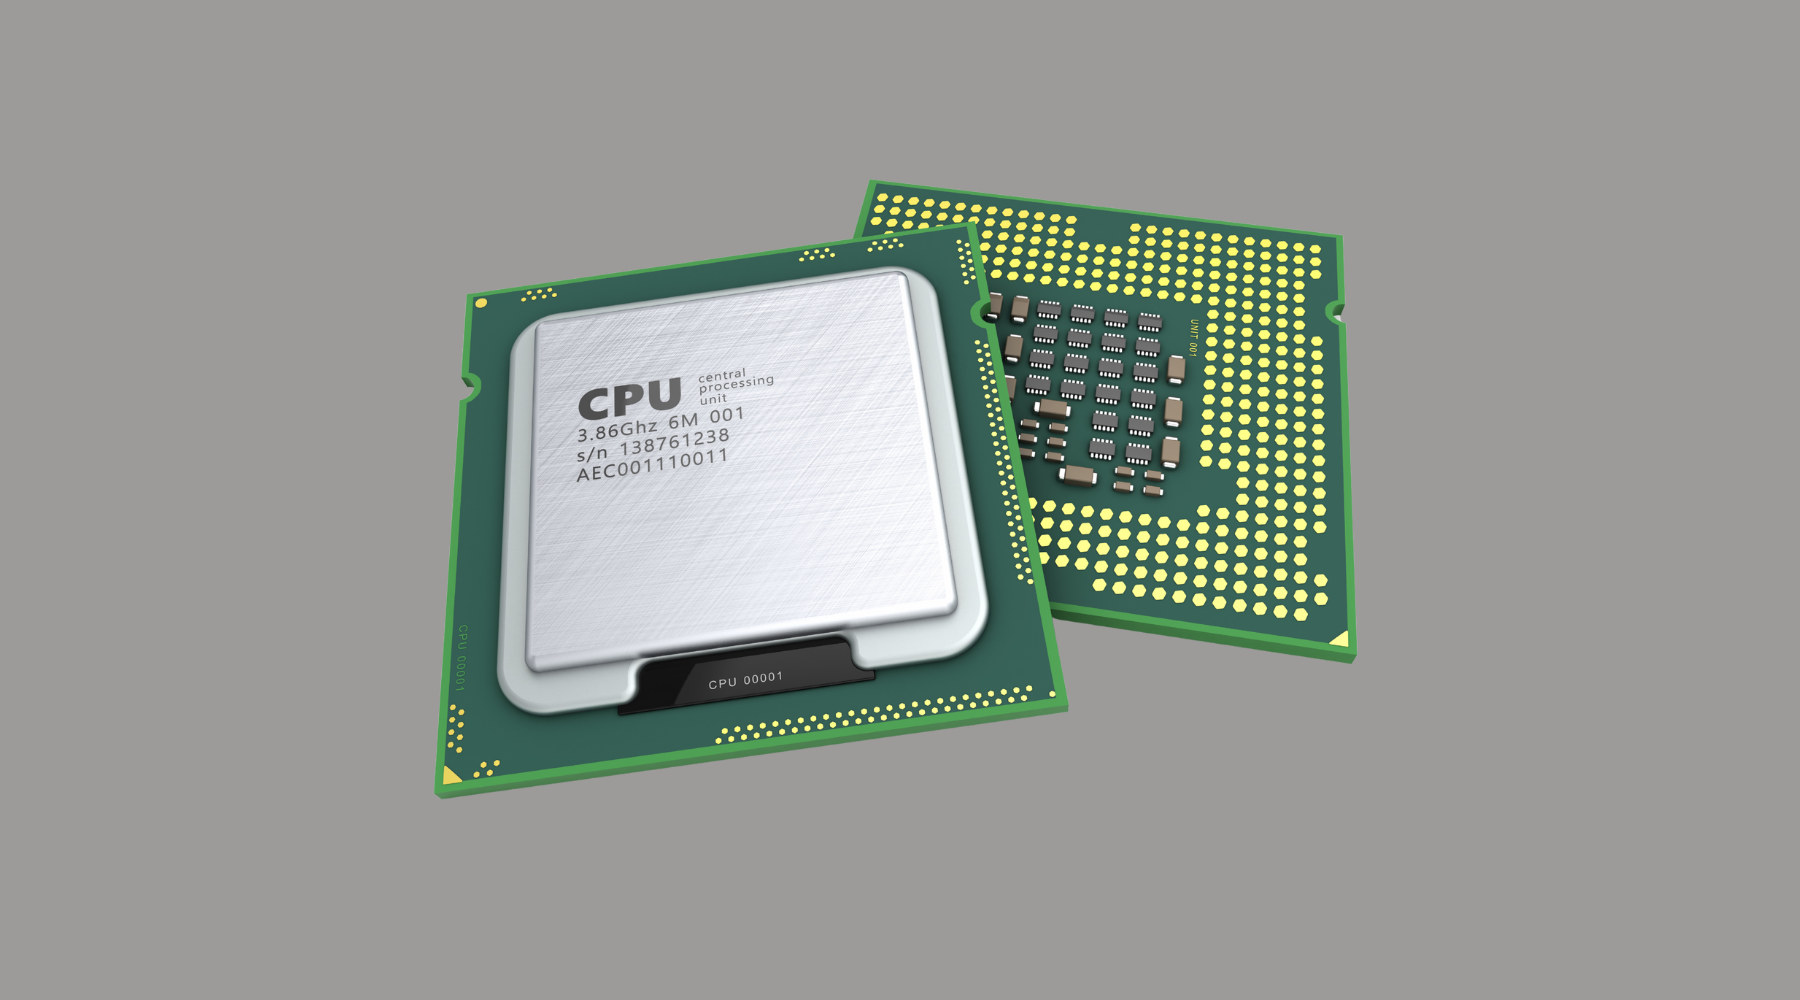
\includegraphics[width=\linewidth]{img/cpu.png}
                \caption{{creata con \href{https://www.canva.com}{Canva}}}
            \end{figure}
    \end{columns}
\end{frame}

\begin{frame}{CPU (Central Processing Unit)}
    \begin{columns}
        \column{.5\textwidth}
            \begin{alertblock}{DEFINIZIONE}
                \begin{minipage}{0.96\linewidth}
                    \justifying
                    I circuiti di temporizzazioni (\textbf{clock}) permettono di generare un segnale ad 
                    onda quadra. Si tratta di un segnale che commuta continuamente da un 
                    livello basso ad uno alto, molti milioni di volte al secondo.\\
                    Per ogni ciclo (\textbf{T}), i circuiti del processore eseguono un'operazione.\\
                    L'\textbf{Hertz} è l'unità di misura della frequenza. I processori attuali 
                    lavorano con clock la cui velocità è di miliardi di hertz (GHz).\\
                    Se T è il periodo di un ciclo, la frequenza è definita come: $f=\frac{1}{T}$\\
                    \bigskip
                    \tiny{\textbf{Curiosità}}\\
                    \tiny{\href{https://www.fastweb.it/fastweb-plus/digital-magazine/processori-multi-core-cosa-sono-e-come-funzionano/}{Processori multi-core}}
                \end{minipage}
            \end{alertblock}
        \column{.5\textwidth}
            \begin{figure}
                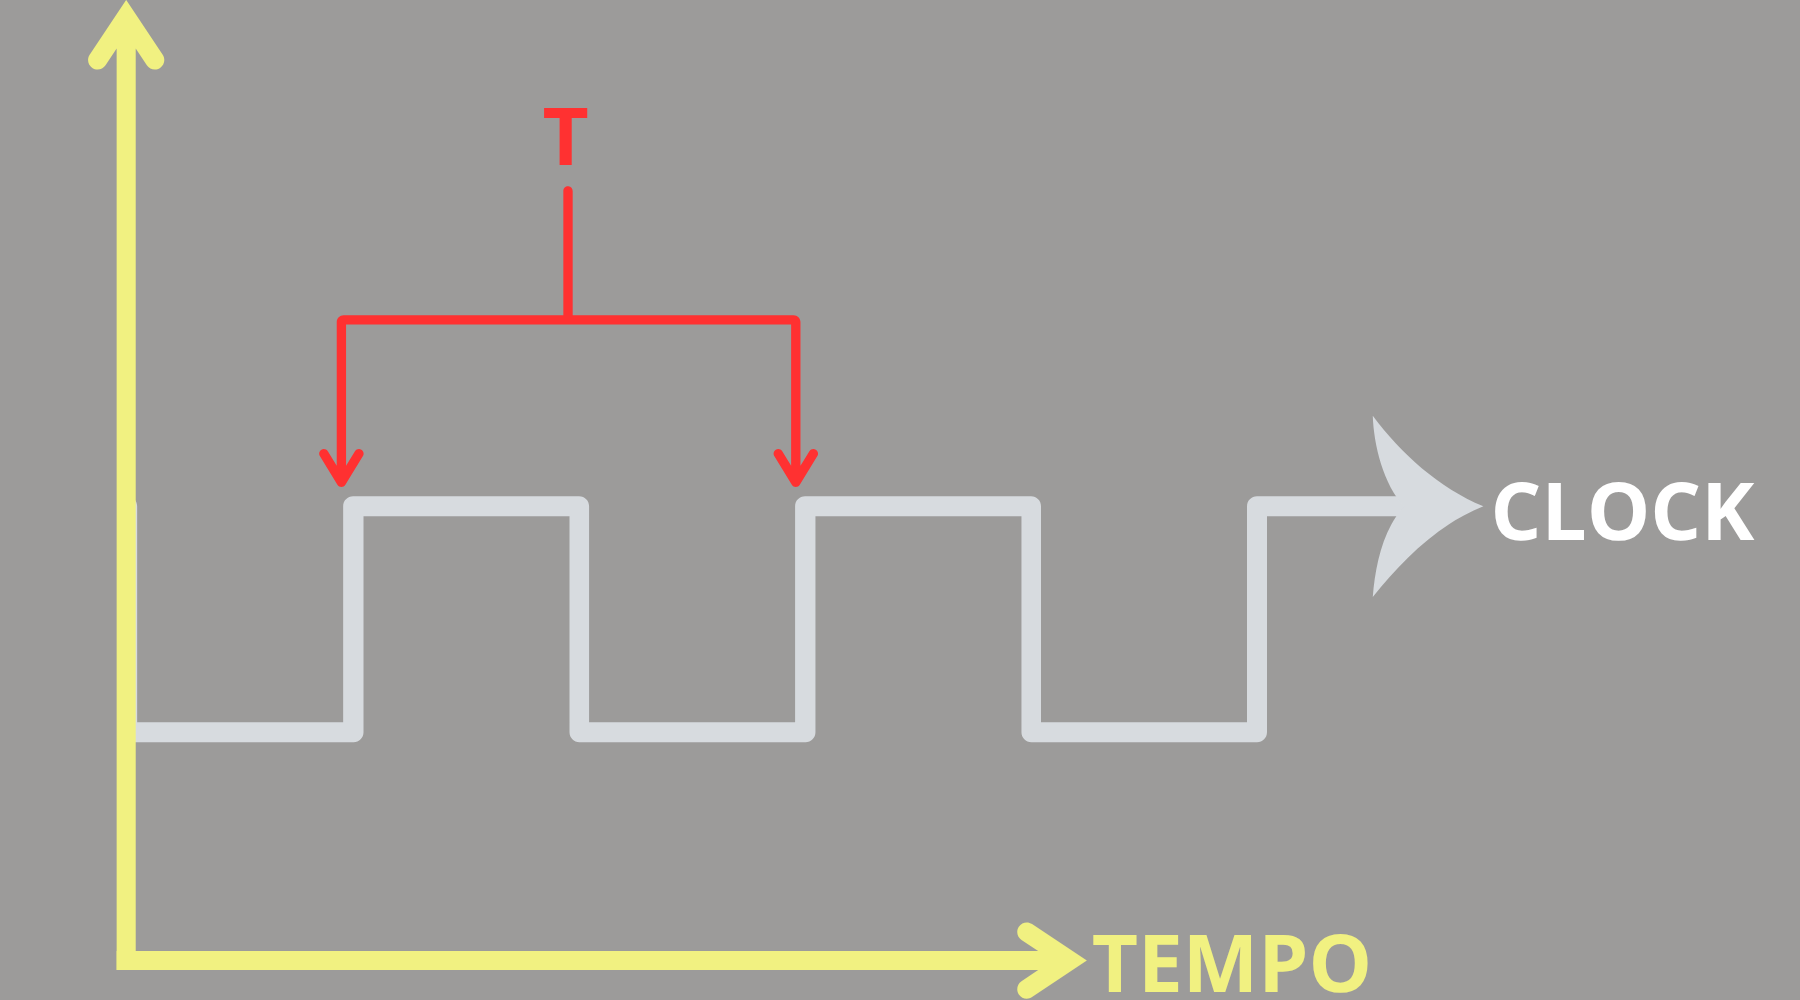
\includegraphics[width=\linewidth]{img/clock.png}
                \caption{{creata con \href{https://www.canva.com}{Canva}}}
            \end{figure}
    \end{columns}
\end{frame}

\begin{frame}{CPU (Central Processing Unit)}
    \begin{columns}
        \column{.5\textwidth}
            \begin{alertblock}{DEFINIZIONE}
                \begin{minipage}{0.96\linewidth}
                    \justifying
                    L'esecuzione di un'istruzione da parte della CPU avviene in tre fasi:
                    \begin{enumerate}
                        \justifying
                        \pause
                        \item \textbf{Fetch}: la CPU preleva l'istruzione da eseguire;
                        \pause
                        \item \textbf{Decode}: la CPU interpreta l'istruzione, ovvero la decodifica per capire quale azione deve compiere;
                        \pause
                        \item \textbf{Execute}: la CPU esegue l'istruzione, ovvero compie l'azione richiesta.
                    \end{enumerate}
                    \bigskip
                    \tiny{\textbf{Curiosità}}\\
                    \tiny{\href{https://www.top500.org/}{Progetto TOP500 per la classifica dei supercomputer}}
                \end{minipage}
            \end{alertblock}
        \column{.5\textwidth}
            \begin{figure}
                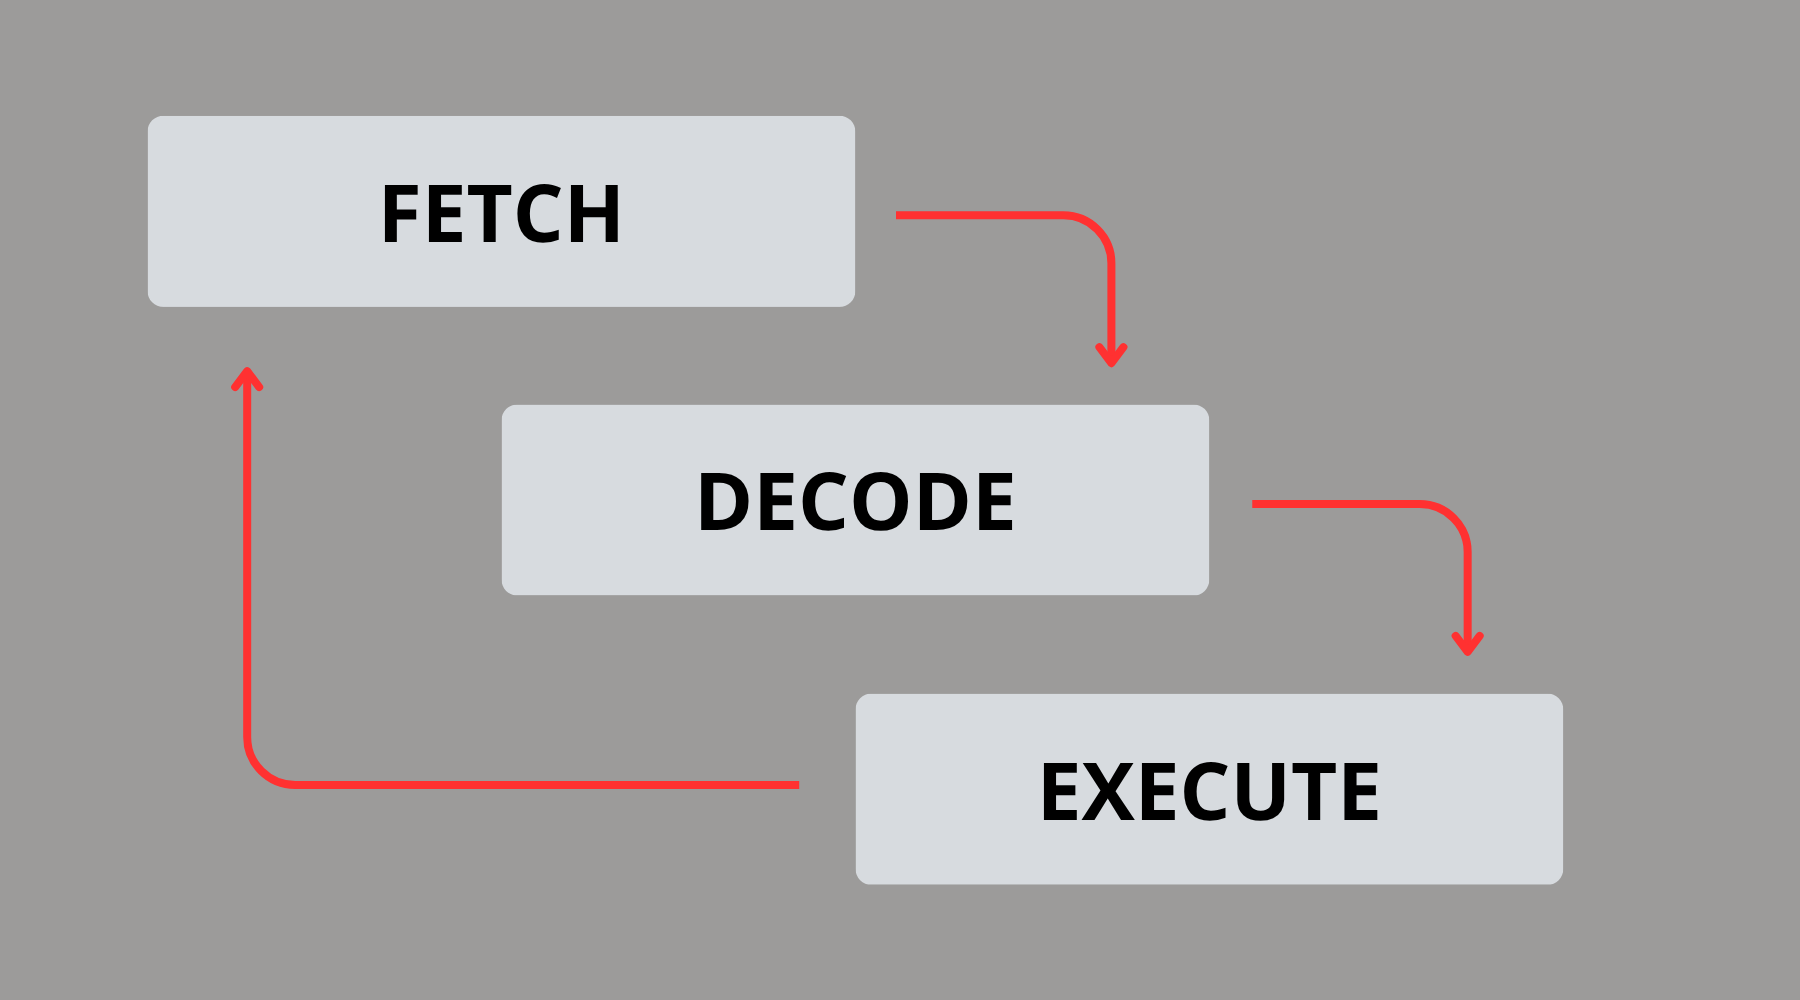
\includegraphics[width=\linewidth]{img/fde.png}
                \caption{{creata con \href{https://www.canva.com}{Canva}}}
            \end{figure}
    \end{columns}
\end{frame}

\section{MEMORIA CENTRALE}

\begin{frame}{MEMORIA CENTRALE}
    \begin{alertblock}{DEFINIZIONE}
        \begin{minipage}{0.98\linewidth}
            \justifying
            Esistono diversi tipi di memoria centrale che differiscono per velocità, capacità, 
            costo e modalità di accesso. Le principali sono:
            \begin{itemize}
                \justifying
                \pause
                \item \textbf{CACHE}: è una memoria estremamente veloce e di piccole dimensioni solitamente 
                installata direttamente all'interno del microprocessore. Nella cache risiedono \textbf{temporaneamente} 
                i dati e le istruzioni che si prevede debbano essere usati nell'immediato futuro.
                \pause
                \item \textbf{ROM (Read Only Memory)}: è una memoria \textbf{di sola lettura permanente}, al suo interno 
                risiedono le istruzioni che permettono l'avvio del sistema operativo.
                \pause
                \item \textbf{RAM (Random Access Memory)}: è una memoria \textbf{VOLATILE}, ovvero i dati in essa contenuti 
                vengono persi quando l'elaboratore viene spento. La RAM è utilizzata per memorizzare i dati e 
                le istruzioni necessarie per l'esecuzione dei programmi in corso.
            \end{itemize}
        \end{minipage}
    \end{alertblock}
\end{frame}

\begin{frame}{MEMORIA CENTRALE}
    \begin{columns}
        \column{.5\textwidth}
            \begin{alertblock}{DDR RAM (Double Data Rate Random Access Memory)}
                \begin{minipage}{0.96\linewidth}
                    \justifying
                    L'espressione \textbf{RAM} significa \textbf{memoria ad accesso casuale}, intendendo con 
                    ciò che il tempo di accesso a una qualsiasi locazione di memoria risulta costante indipendentemente 
                    dalla posizione dell'area di memoria considerata.\\
                    I chip di RAM oggi sono identificati con la sigla \textbf{DDR} (\textbf{Double Data Rate}), che indica 
                    la capacità di trasferire i dati al processore sia sul fronte di salita che di discesa 
                    del segnale di clock, quindi due volte per ciclo.
                \end{minipage}
            \end{alertblock}
        \column{.5\textwidth}
            \begin{figure}
                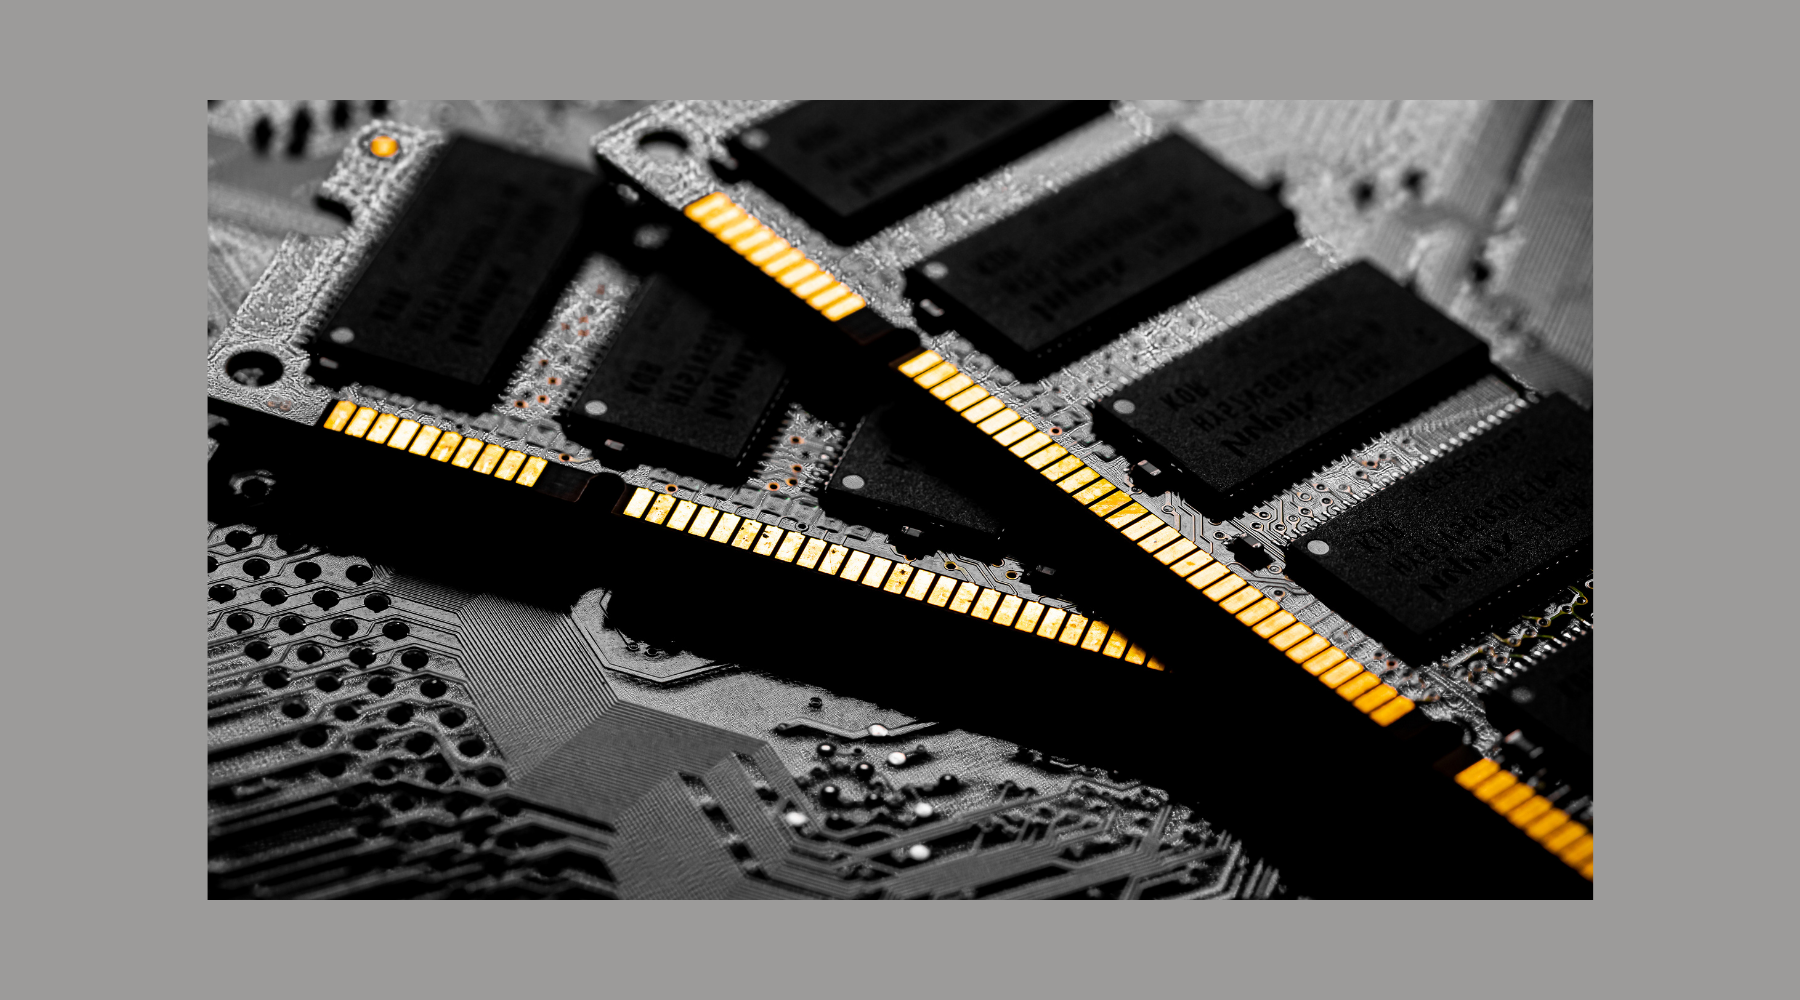
\includegraphics[width=\linewidth]{img/ram.png}
                \caption{{creata con \href{https://www.canva.com}{Canva}}}
            \end{figure}
    \end{columns}
\end{frame}

\section{SCHEDA MADRE}

\begin{frame}{SCHEDA MADRE}
    \only<1 | handout:1>{\begin{figure}
        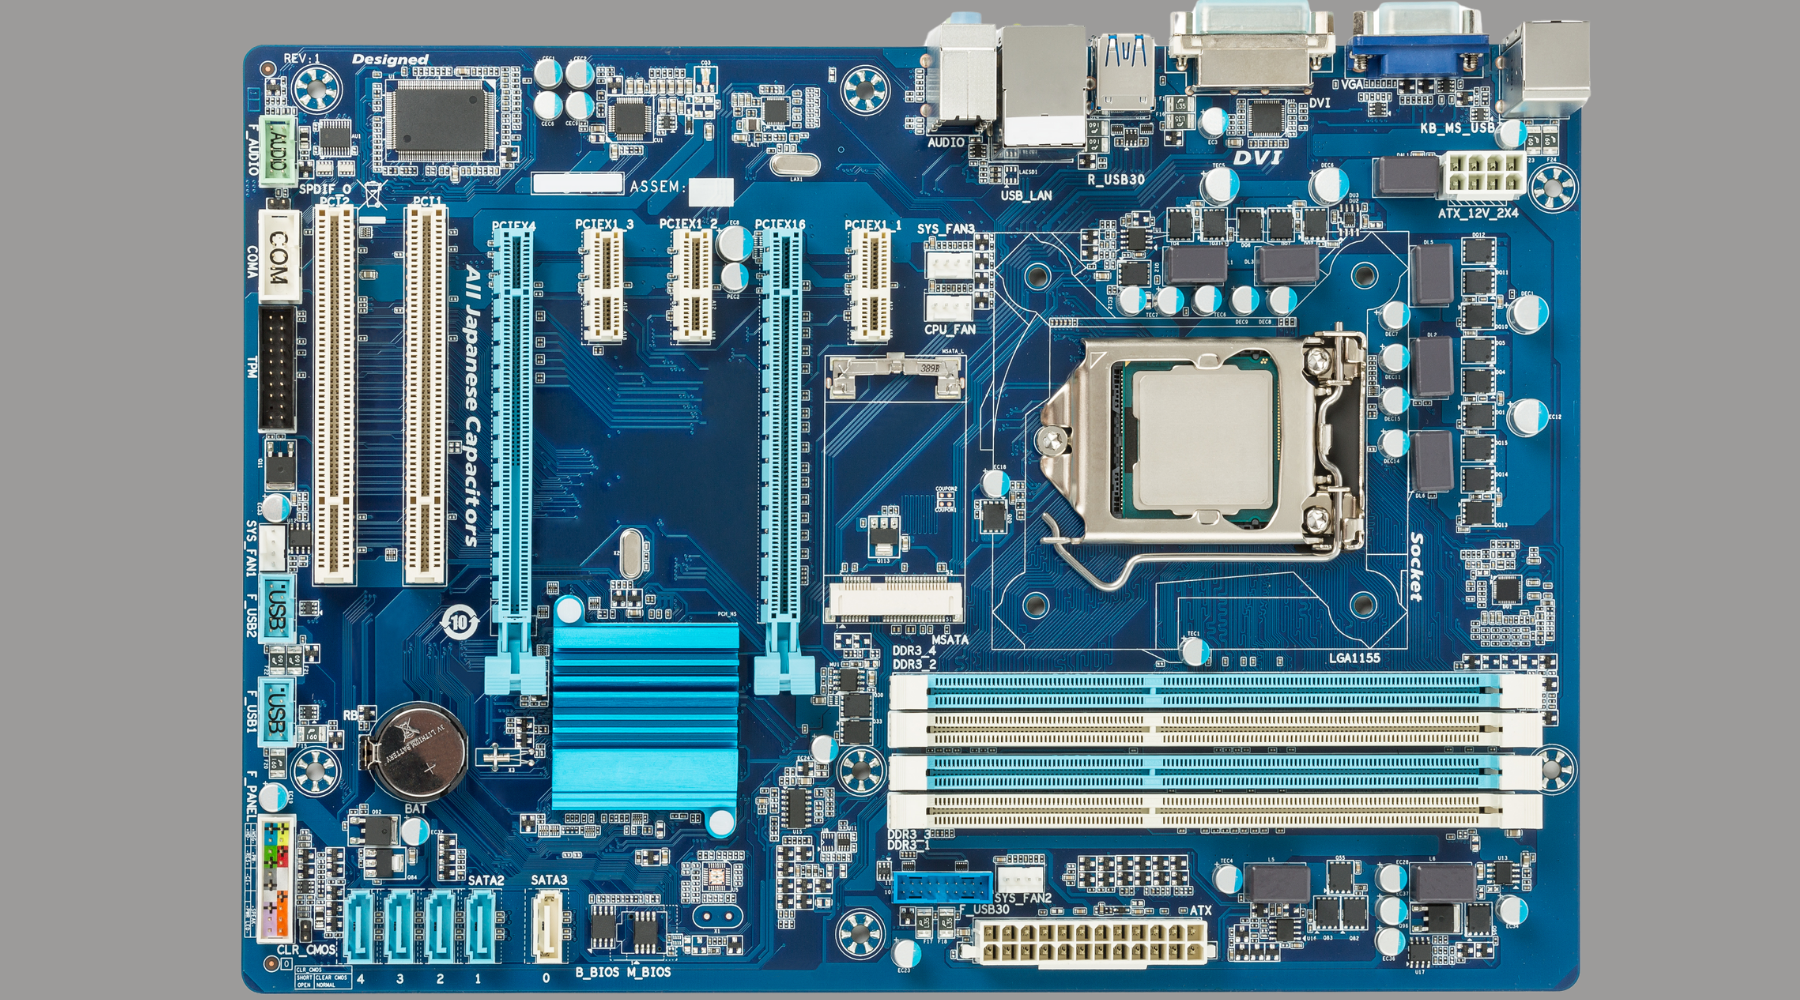
\includegraphics[width=\linewidth]{img/schedaMadre1.png}
        \caption{{creata con \href{https://www.canva.com}{Canva}}}
    \end{figure}}
    \only<2 | handout:0>{\begin{figure}
        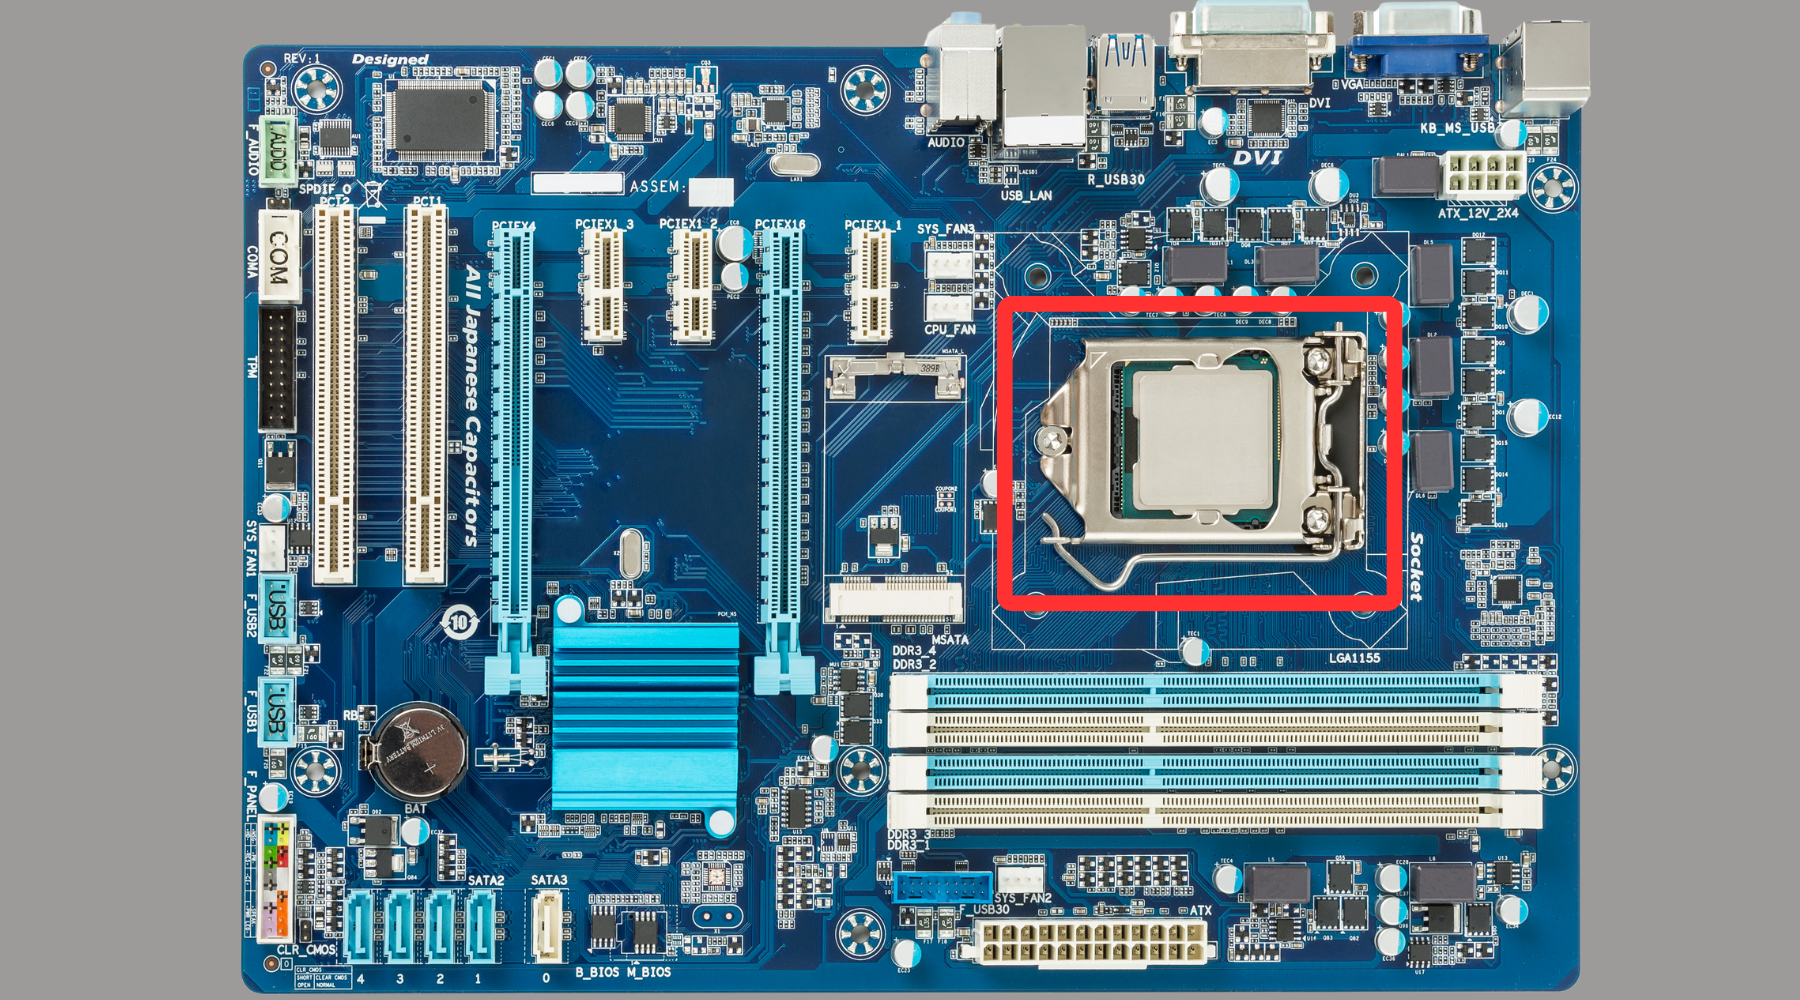
\includegraphics[width=\linewidth]{img/schedaMadre2.png}
        \caption{{creata con \href{https://www.canva.com}{Canva}}}
    \end{figure}}
    \only<3 | handout:0>{\begin{figure}
        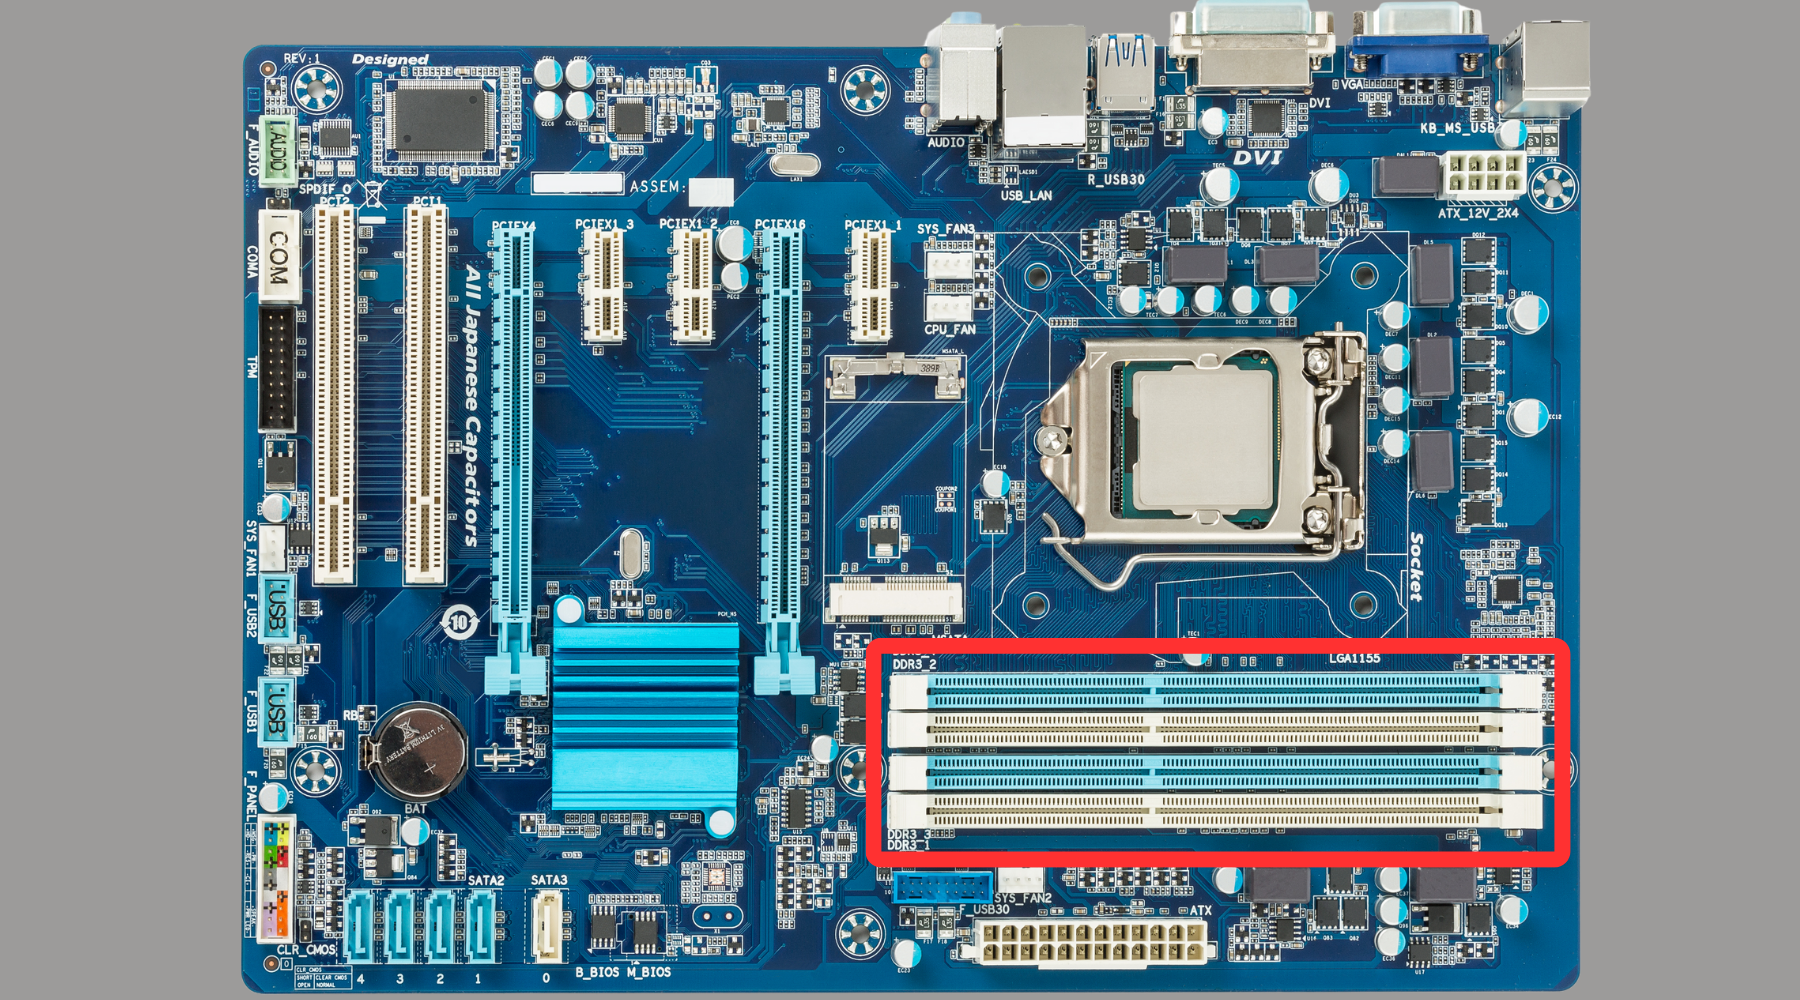
\includegraphics[width=\linewidth]{img/schedaMadre3.png}
        \caption{{creata con \href{https://www.canva.com}{Canva}}}
    \end{figure}}
    \only<4 | handout:0>{\begin{figure}
        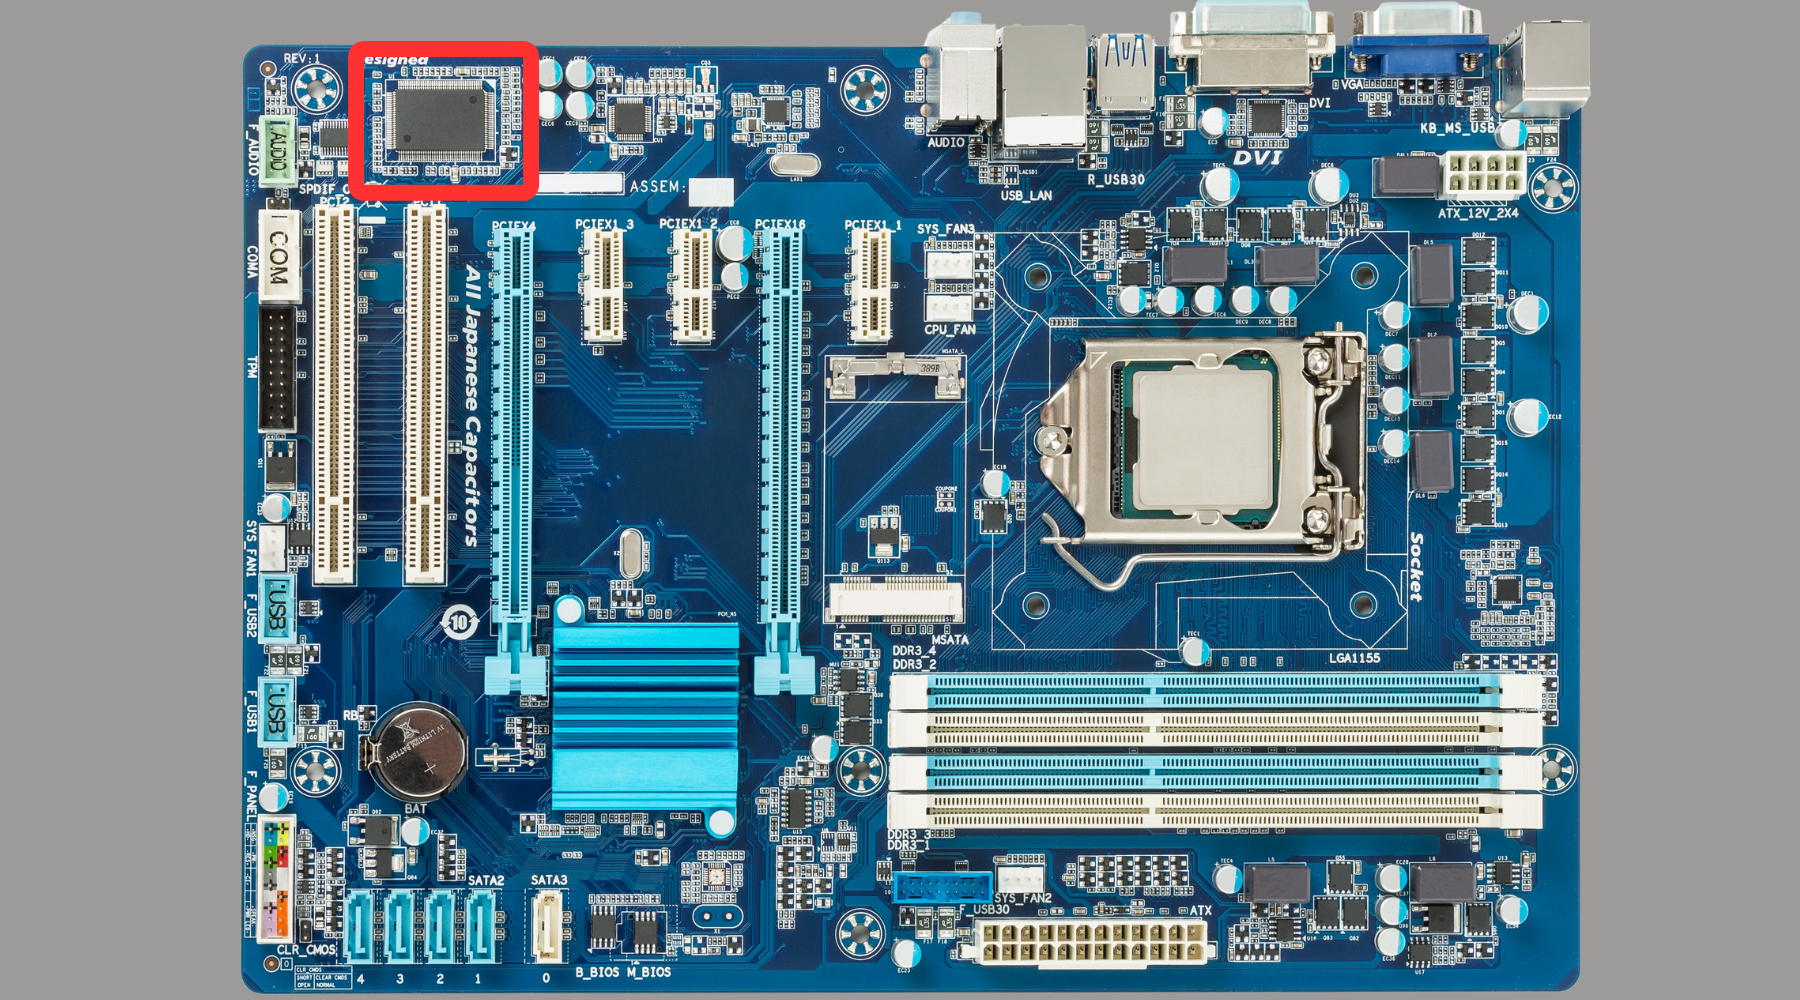
\includegraphics[width=\linewidth]{img/schedaMadre4.png}
        \caption{{creata con \href{https://www.canva.com}{Canva}}}
    \end{figure}}
    \only<5 | handout:0>{\begin{figure}
        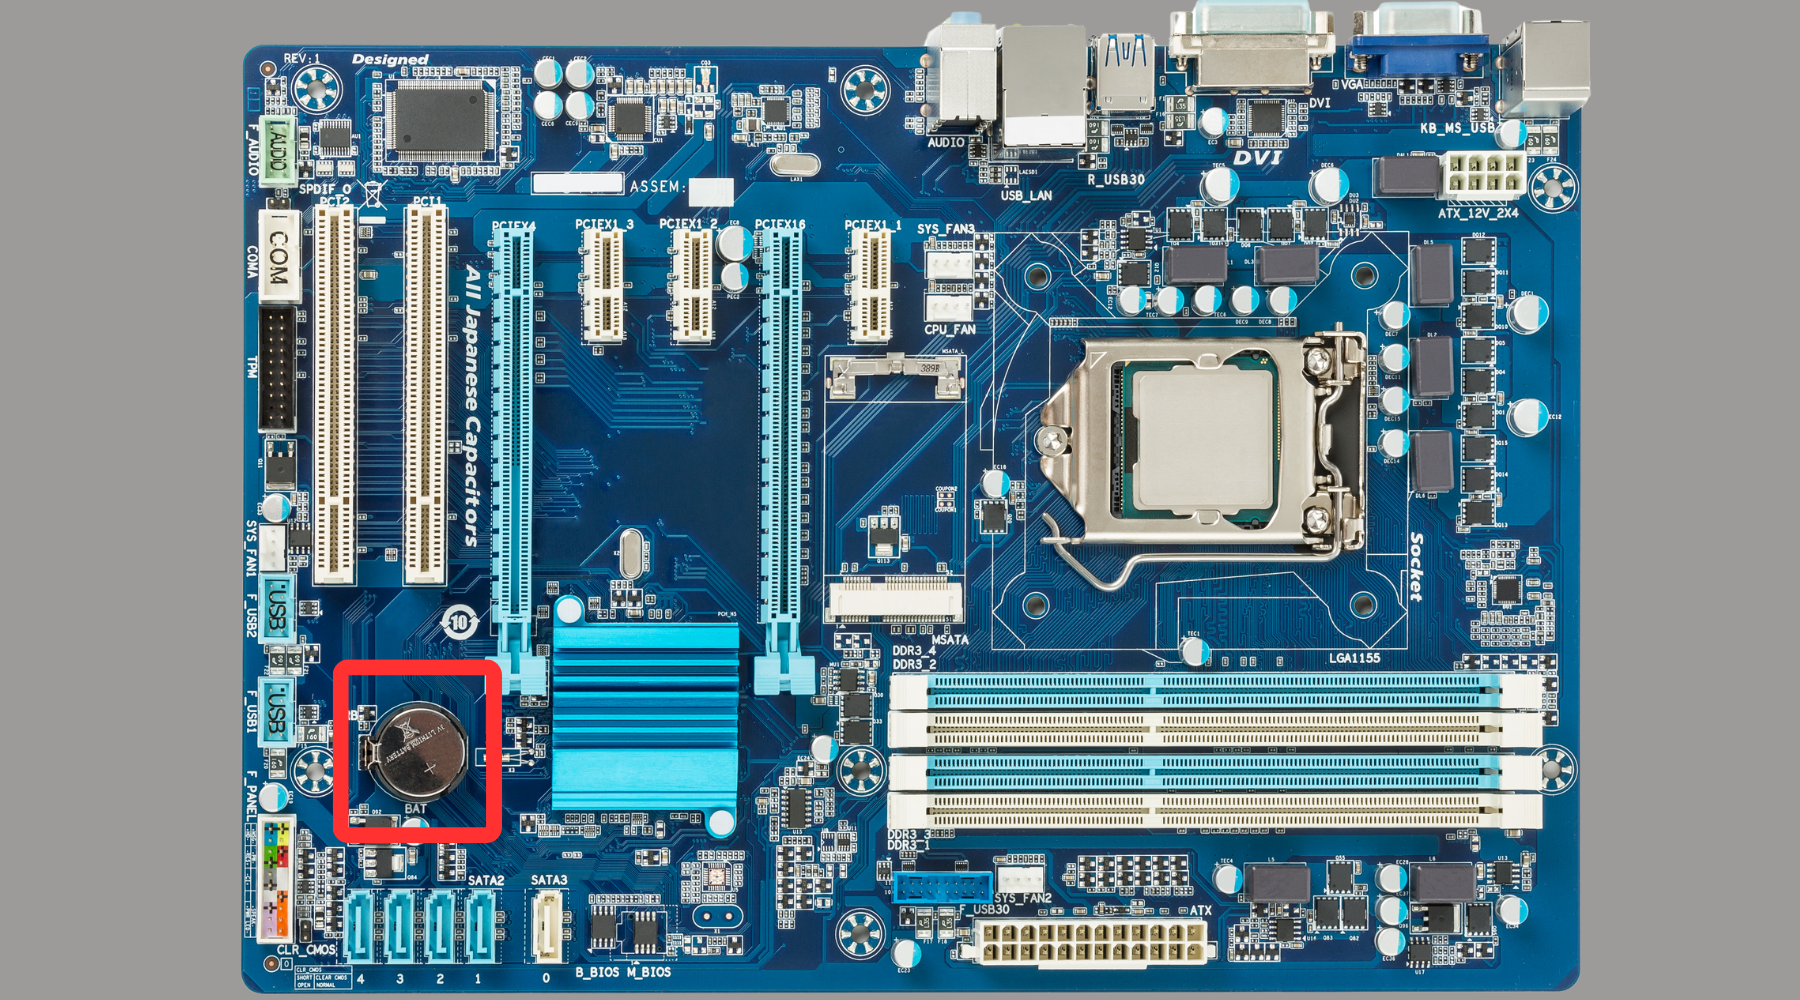
\includegraphics[width=\linewidth]{img/schedaMadre5.png}
        \caption{{creata con \href{https://www.canva.com}{Canva}}}
    \end{figure}}
\end{frame}

\section{PERIFERICHE INPUT/OUTPUT}

\begin{frame}{PERIFERICHE}
    \begin{alertblock}{DEFINIZIONE}
        \begin{minipage}{0.98\linewidth}
            \justifying
            Le periferiche sono un insieme di apparati molto eterogeneo per costo, funzionalità, modalità 
            di interazione con l'elaboratore e con l'utente, e possono essere classificate in:
            \bigskip
            \begin{itemize}
                \justifying
                \pause
                \item \textbf{Periferiche di input}: permettono di inserire dati e comandi nell'elaboratore agendo in 
                modo unidirezionale, ovvero dall'utente verso l'elaboratore (\textbf{INGRESSO}).
                \pause
                \item \textbf{Periferiche di output}: permettono di visualizzare o riprodurre i risultati dell'elaborazione 
                agendo in modo unidirezionale, ovvero dall'elaboratore verso l'utente (\textbf{USCITA}).
                \pause
                \item \textbf{Periferiche di input/output}: permettono sia di inserire dati che di visualizzare 
                i risultati dell'elaborazione agendo in modo bidirezionale.
            \end{itemize}
            \bigskip
        \end{minipage}
    \end{alertblock}
\end{frame}

\section{MEMORIE DI MASSA}

\begin{frame}{MEMORIE DI MASSA}
    \begin{alertblock}{DEFINIZIONE}
        \begin{minipage}{0.98\linewidth}
            \justifying
            ``Le memorie di massa hanno lo scopo di memorizzare grandi quantità di informazioni in modo 
            permanente e per questa caratteristica sono definite \textbf{NON VOLATILI}. A differenza della 
            memoria centrale, presentano il vantaggio di mantenere il loro contenuto anche in assenza di 
            alimentazione elettrica e possono memorizzare una quantità di dati anche mille vole superiore; 
            \textbf{i tempi di accesso ai dati sono però notevolmente superiori}.''\\
            \bigskip
            \tiny{\textbf{Fonte}}\\
            \tiny{\href{https://catalogo.sanoma.it/si-op-104157-dal-bit-all-intelligenza-artificiale.html}{Dal BIT all'INTELLIGENZA ARTIFICIALE}}
        \end{minipage}
    \end{alertblock}
\end{frame}

\section{COMPRARE UN PC O UNO SMARTPHONE}

\begin{frame}{COMPRARE UN PC O UNO SMARTPHONE}
    \begin{enumerate}
        \justifying
        \item \textbf{Definire il budget}: stabilire quanto si è disposti a spendere per l'acquisto;
        \pause
        \item \textbf{Definire l'uso}: stabilire per quale scopo si sta acquistando il dispositivo;
        \pause 
        \item \textbf{Scegliere le specifiche hardware}: analizzare le specifiche tecniche del dispositivo, 
        confrontando le caratteristiche dei vari modelli e marchi disponibili e tenendo in considerazione 
        anche le recensioni e le opinioni degli utenti.
    \end{enumerate}
    \bigskip
    \tiny{\textbf{Curiosità}}\\
    \tiny{\href{https://versus.com/it}{Versus: sito di confronto tra prodotti}}
\end{frame}

\end{document}